

\section{Implementation Approach}
To validate the applicability and efficacy of our proposed solution (based on lightweight cryptographic algorithms), we conducted an experiment using an ESP32 -- a resource-constrained IoT device -- and Ditto -- an open-source framework for building Digital Twin \footnote{https://eclipse.dev/ditto/}. We opt for ESP32 boards for the experiment due to the fact that they are low-cost and low-power devices in the market \cite{maier_comparative_2017}. Ditto was selected for its ease of customization through Java-based plugins and its widespread use in the open-source community. 



\begin{figure}[H]
    \centering
    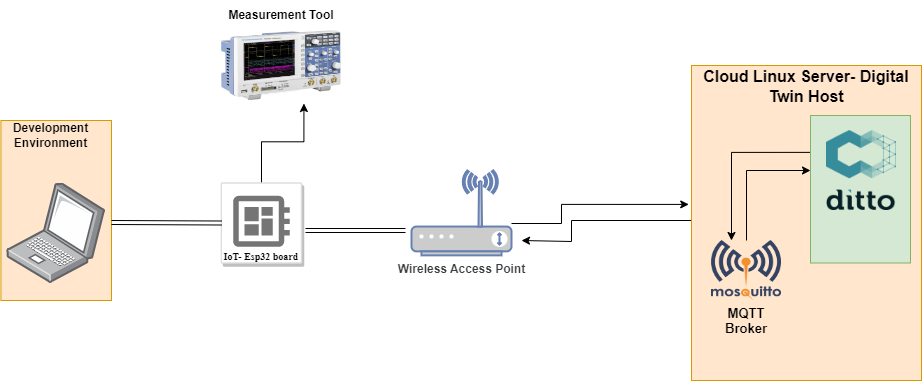
\includegraphics[width=\textwidth]{images/fp/experiment.drawio.png}
    \caption{Research Experiment Setup}
    \label{fig:experiment-setup}
\end{figure}

This section provides a detail of the experimental setup (of Fig \ref{fig:experiment-setup}) and implementation detail of the lightweight encryption/authentication algorithm implemented on both the constrained device and the Digital Twin framework.



% ======================================================================================================
% NOTES, TODOS
% What is Ditto -> reference the official webisite

% ======================================================================================================

\subsection{Eclipse Ditto - Digital Twin Setup}
Eclipse Ditto is an open-source framework for managing IoT devices to create Digital Twin \cite{noauthor_eclipse_nodate}.
It integrates devices via layers like Eclipse Hono and MQTT brokers, allowing managed Digital Twins to connect with various backend systems using protocols such as AMQP, Apache Kafka, HTTP, and MQTT. 

Ditto can be deployed on-premises or in the cloud. For this research, we build and deploy the Ditto code base in the cloud.
In addition, We have two options for deploying and running Ditto on a cloud Linux server. The first option involves utilizing the Kubernetes cluster, which necessitates substantial infrastructure resources. Specifically, a minimum of 4 GB RAM, 8 core processes, and 20 GB disk storage are required. However, the second option, which we have chosen, involves using Docker. This alternative demands fewer resources compared to the previous one. 

Running Ditto in a docker container have seven microservices operating in parallel, each fulfilling distinct functions. These microservices include \textit{Nginx} as the web server, \textit{}, \textit{Ditto Connectivity} for managing the device-to-Ditto connectivity, \textit{Ditto Thing} for managing things (counterpart of physical devices), \textit{Thing Search} for facilitating efficient search using MongoDB, \textit{Swagger-UI} for providing a web-based user interface, and \textit{Ditto Policies} for mainting controlled access over things.

The following steps outline the process required to set up Ditto on a Linux server:

\begin{itemize}
    \item \textbf{Install and Configure Docker:} Begin by installing Docker, a platform for creating and managing containers. Ensure Docker Compose, a utility for defining and running multi-container applications is also installed and configured on your Linux server.
    \item \textbf{Clone Ditto Codebase:} Access the official GitHub repository for Eclipse Ditto and clone the codebase using the command: git clone\texttt{https:// github.com/eclipse-ditto/ditto.git}. 
    \item \textbf{Deploy Ditto Microservices:} Start the Ditto cluster by deploying its microservices in containers. Execute the command: docker-compose up -d. 
    \item \textbf{Check Microservices Status:} verify that all microservices are running and check the health status of Ditto using the following commands: curl -u devops:foobar http://localhost:8080/status/health
\end{itemize}



The process of running Ditto and connecting with the MQTT broker is described below.

\textit{Creating Policy}: In Ditto policies are JSON configuration file that defines who access what. Creating policies is the first step in running Ditto. The policy configuration we use for our project is presented as follows. To speed up experimenting with Ditto we used a bash script that we can run from the terminal of the server. 
\begin{lstlisting}[style=CStyle, caption={A Bash Script of Ditto command To Create Connection}]
#!/bin/bash

curl -X PUT 'http://localhost:8080/api/2/policies/ut.thesis.demo:policy' -u 'ditto:ditto' -H 'Content-Type: application/json' -d '{
    "entries": {
        "owner": {
            "subjects": {
                "nginx:ditto": {
                    "type": "nginx basic auth user"
                }
            },
            "resources": {
                "thing:/": {
                    "grant": [
                        "READ","WRITE"
                    ],
                    "revoke": []
                },
                "policy:/": {
                    "grant": [
                        "READ","WRITE"
                    ],
                    "revoke": []
                },
                "message:/": {
                    "grant": [
                        "READ","WRITE"
                    ],
                    "revoke": []
                }
            }
        }
    }
}'
\end{lstlisting}

\textit{Creating things}: Things are the digital representation of the physical device with attributes and features. Like we did for policy, for the thing we also created bash script as follow. 

\begin{lstlisting}[style=CStyle, caption={A Bash Script To Create Things in Ditto}]
    

#!/bin/bash

curl -X PUT 'http://localhost:8080/api/2/things/ut-sensors:esp01' -u 'ditto:ditto' -H 'Content-Type: application/json' -d '{
    "policyId": "ut.thesis.demo:policy",
    "attributes": {
        "name": "Esp3201",
        "type": "Esp32 board"
    },
    "features": {
        "temperature": {
            "properties": {
                "value": 0
            }
        },
        "altitude": {
            "properties": {
                "value": 0
            }
        }
    }
}'
\end{lstlisting}

\textit{Creating connection:} The connection configuration file serves the purpose of defining the source and target of the MQTT broker topic. In this case, the connection type is MQTT, and the specified URI contains the IP address. The source topic is set as "ut-sensors/\#", indicating that Ditto will receive data from the broker when a message is published on any topic under "ut-sensors". On the other hand, the target address is defined as "ut-sensors/{{thing:id}}", which means that Ditto will publish data on the corresponding topic of the device whenever an event is emitted by the thing with the given ID. The inclusion of "\#" at the end of the string signifies that messages can be received from any topic under "ut-sensors". This configuration enables bidirectional communication and data exchange between Ditto and IoT devices via the MQTT broker. 

\begin{lstlisting}[style=CStyle, caption={A Bash Script to Create Connection in Ditto}]
#!/bin/bash

curl -X POST 'http://localhost:8080/devops/piggyback/connectivity?timeout=10' -u 'devops:foobar' -H 'Content-Type: application/json' -d '{
    "targetActorSelection": "/system/sharding/connection",
    "headers": {
        "aggregate": false
    },
    "piggybackCommand": {
        "type": "connectivity.commands:createConnection",
        "connection": {
            "id": "ascon-ut-mqtt-connection",
            "connectionType": "mqtt",
            "connectionStatus": "open",
            "failoverEnabled": true,
            "uri": "tcp://<IP address>:1883",
            "sources": [{
                "addresses": ["ut-sensors/#"],
                "authorizationContext": ["nginx:ditto"],
                "qos": 0,
                "filters": [],
                                "headerMapping": {},
                                "payloadMapping": ["AsconPayload"],
                                "replyTarget": {
                                        "headerMapping": {},
                                        "expectedResponseTypes": [
                                          "response",
                                          "error"
                                        ],
                                        "enabled":false
                                }
            }],
                        "targets": [{
                                "address": "ut-sensors/{{ thing:id }}",
                                "topics": [
                                "_/_/things/twin/events",
                                "_/_/things/live/messages"
                                ],
                                "authorizationContext": ["nginx:ditto"],
                                "headerMapping": {},
                "qos": 0,
                "payloadMapping": ["AsconPayload"]
                        }]
        }
    }
}'
\end{lstlisting}


Another crucial component that works hand in hand with Ditto is the MQTT broker. In the subsequent section, we will deep dive into the detailed process of setting it up and initiating its operation.

\subsection{Building MQTT Broker (Mosquitto) from Source}

The MQTT broker is a lightweight protocol designed for IoT communication[ref]. In our project, we utilized the MQTT implementation from Eclipse Ditto, specifically Mosquitto. To ensure full control and customization, we built the MQTT implementation from the source on our Linux server. This approach was undertaken primarily to accommodate the implementation of the lightweight encryption algorithm into the source code. However, we later decided to implement the algorithms by extending the ditto source code itself through the connectivity extension provided. 

In order to run the MQTT broker on our Linux server, there are a few necessary steps to follow. Firstly, we need to install a couple of dependencies, namely \texttt{libcjson-dev and libwebsocket-dev}. Once these dependencies are installed, we proceed to build the source code by executing the following command: 

\texttt{make WITH\_SRV=yes WITH\_TLS=no WITH\_WEBSOCKETS=yes WITH\_CJSON = yes WITH\_BUNDLED\_DEPS = yes WITH\_DOCS=no}. After the build process, we can verify the successful installation of MQTT by running the tests using the command \texttt{make test}. Finally, to complete the installation, we execute \texttt{sudo make install} to install the MQTT broker into our system. 


It is worth noting that the MQTT broker can be installed either on the same machine as the Ditto running machine or on a different remotely accessible machine. Our proposed scheme ensures secure communication between the IoT device and the cloud-hosted Ditto service. The MQTT broker has limited visibility, as it can only access the encrypted payload, thereby preventing any malicious broker from compromising the security of the communication. The lightweight authentication and encryption algorithm we leverage into our proposed solution guarantees the confidentiality and integrity of the data exchanged.

To start the MQTT service, there are two options available. The first option is to execute the command "mosquitto" directly. Alternatively, we can start the MQTT service with additional configuration options by specifying the configuration file path using the following command: "mosquitto -v -c /path/to/mosquitto.conf".

To publish and subscribe to topics using the MQTT broker, we utilize the commands provided on the GitHub page of Mosquitto. 
    \begin{itemize}
        \item For subscribing to a topic, we employ the command "mosquitto\_sub -t 'test/topic' -v". This command enables us to subscribe to the specified topic and receive the messages associated with it. 
        \item To publish a message to a topic, we run "mosquitto\_pub -t 'test/topic' -m 'hello world'". By executing this command, we can publish a message to the specified topic so that other subscribers to the topic get notified. 
    \end{itemize}
    
    
% \begin{figure}[H]
%     \caption{Ditto Architecture}
%     \centering
%     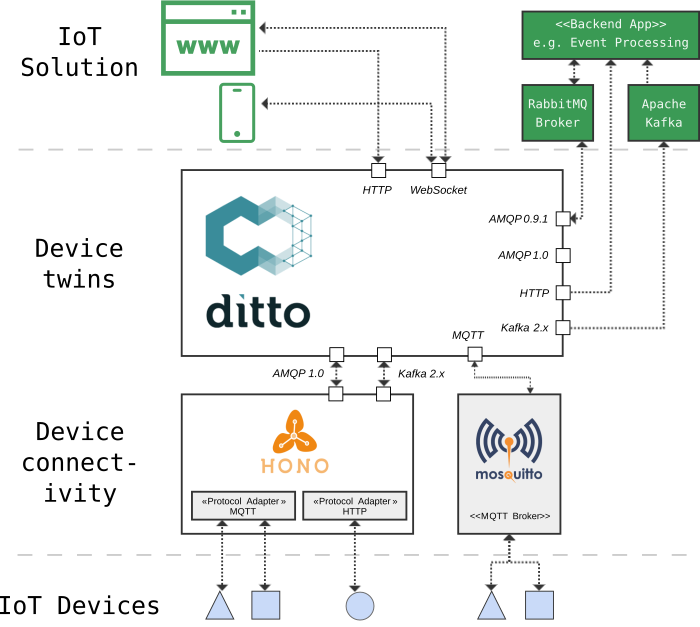
\includegraphics[width=\textwidth]{images/fp/ditto-overview-1.png}
%     \label{fig:ditto-arch}
% \end{figure}




\subsection{Implementation of ASCON and AES-GCM for device}


The implementation of both algorithms on the hardware IoT device was carried out using C and C++ programming languages within Arduino for esp-idf embedded development framework. We opted for C and C++ because those two choices are more suitable for low-level programming such as for embedded resource constraint devices. The main application for the IoT device was developed in C++, while the algorithm for ASCON and AES-GCM was implemented in C and incorporated through the use of the "extern" macro in C++ main application.


The counterpart of the algorithms in the digital twin was implemented in Java. This is because the connectivity microservice of Ditto is implemented in Java. This allowed us to extend the connectivity module using Java to incorporate an extension for encryption and decryption of the payload that comes from IoT devices.

It is worth noting that we neither altered nor introduced optimizations in the design of these algorithms. For both algorithms (ASCON\footnote{https://github.com/ascon/ascon\_collection} and AES-GCM\footnote{https://github.com/usnistgov/Lightweight-Cryptography-Benchmarking/tree/main /implementations/\_reference\_/crypto\_aead/aes-gcm/mbedtls}), we selected the optimized reference implementations tailored for the ESP32 device chip. However, to enhance the security of our implementation, we incorporated a function to generate a nonce. This aspect is crucial in addressing vulnerabilities such as replay attacks, which involve the repeated use of encrypted information.








\subsection{Ditto Java Base Payload Mapping}

In the context of Eclipse Ditto, data storage and transfer are facilitated through a format known as the Ditto protocol. This protocol utilizes a JSON structure, employing key-value pairs to represent and transmit information.

To seamlessly integrate with Ditto's capabilities, the connectivity microservice bundled with Ditto offers an extension specifically designed for intercepting incoming data. This extension allows for the mapping of data from its original form to a format that Ditto can understand and store in its underlying MongoDB database. Using the Ditto payload mapping feature, we can decrypt incoming encrypted payload messages and convert them into a format that Ditto can process and store.
 
With the payload mapping feature in Ditto's connectivity microservice, we can do the following: receive encrypted data from the IoT device, decrypt and authenticate it, and convert it into Ditto protocol messages. This helps ensure that the data sent between the IoT device and Ditto is secure and authentic.

To implement our custom mapping functionality to encrypt and decrypt, we perform the following steps:
\begin{itemize}
    \item[-] Implement and build a Java class as Jar file for the encryption and decryption functionality. This class will provide the ASCON or AES-GCM encryption and decryption operations needed for secure communication and data handling. 
    \item[-] Develop a custom message mapper class that will handle the conversion of incoming device messages to the appropriate Ditto protocol format. This class will integrate with the aforementioned encryption and decryption functionality to ensure data integrity and security during the mapping process.
    \item[-]Configure the Ditto connectivity microservice to recognize and load our custom message mapper. This configuration step ensures that incoming messages are routed to our custom mapper for processing, enabling seamless integration of our specific data transformation requirements within the Ditto framework.
\end{itemize}









\subsection{Sending Authenticated Encrypted Payload To Ditto}
\label{sec:sendingauth}

This section demonstrates the proof of concept securing the communication between the IoT device and the Digital Twin (Ditto). 

Figure \ref{fig:log-mon} depicts a snapshot captured from the serial monitor output of the board (device) utilizing PlatformIO (embedded development framework). The image showcases the device transmitting an encrypted payload to the 'ut-sensors' topic while including additional data labeled as 'tid' to uniquely identify the device. 

In Figure \ref{fig:wireshark}, a captured packet during the communication is displayed. Upon observation, it becomes evident that the topic being utilized is 'ut-sensors', and the message section of the MQTT protocol header contains the device identifier along with the encrypted payload.


\begin{figure}[H]
   
    \begin{subfigure}[c]{1\linewidth}
        \centering
        
        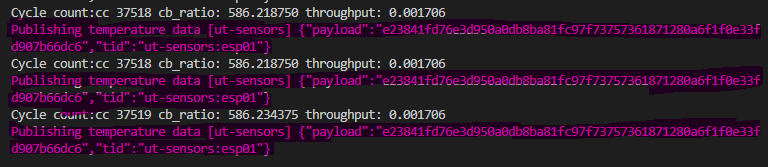
\includegraphics[width=\linewidth]{images/fp/serialport.png}
        \caption{Log Output of ESP32 Device Using Serial Monitor}
        \label{fig:log-mon}
     \end{subfigure}    

    \begin{subfigure}[c]{1\linewidth}
        \centering
        
        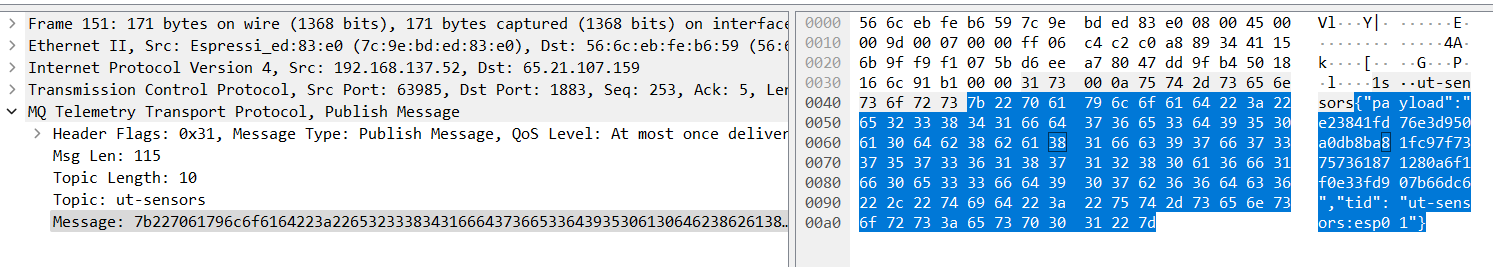
\includegraphics[width=\linewidth]{images/fp/wireshark.png}
        \caption{Wireshark Captured MQTT Communication From IoT to Ditto}
        \label{fig:wireshark}
    \end{subfigure}
     \caption{Serial Monitor of ESP32 Board and Wireshark Capturing Communication Between The Device and Ditto(DT)}
\end{figure}

The MQTT broker, hosted on the same server with Ditto, acts as a proxy, facilitating the transmission of authenticated and encrypted payloads through a publish-subscribe model. Once the MQTT broker receives a payload, it  notifies Ditto of the new message it has subscribed to. Ditto then retrieves the payload, decrypts it, and maps it into a Ditto protocol message, which is subsequently stored in a database.

To simulate the life cycle of a Digital Twin, we have developed a small web application that models the temperature and humidity features of an ESP32 sensor. The application utilizes JavaScript to retrieve these values through a stream of emissions using server-side events (SSE). Moreover, to send commands or messages to the server, we employ the HTTP POST API of Ditto. By subscribing to the command event associated with a specific topic, any device can consume the message and execute the corresponding action. This activity effectively simulates the communication between the digital twin and the actuators. Conversely, the communication from the (I)IoT device to the Digital Twin serves the purpose of collecting telemetry data from the operational environment.

\begin{figure}[H]
   
    \begin{subfigure}[c]{1\linewidth}
        
        \centering
        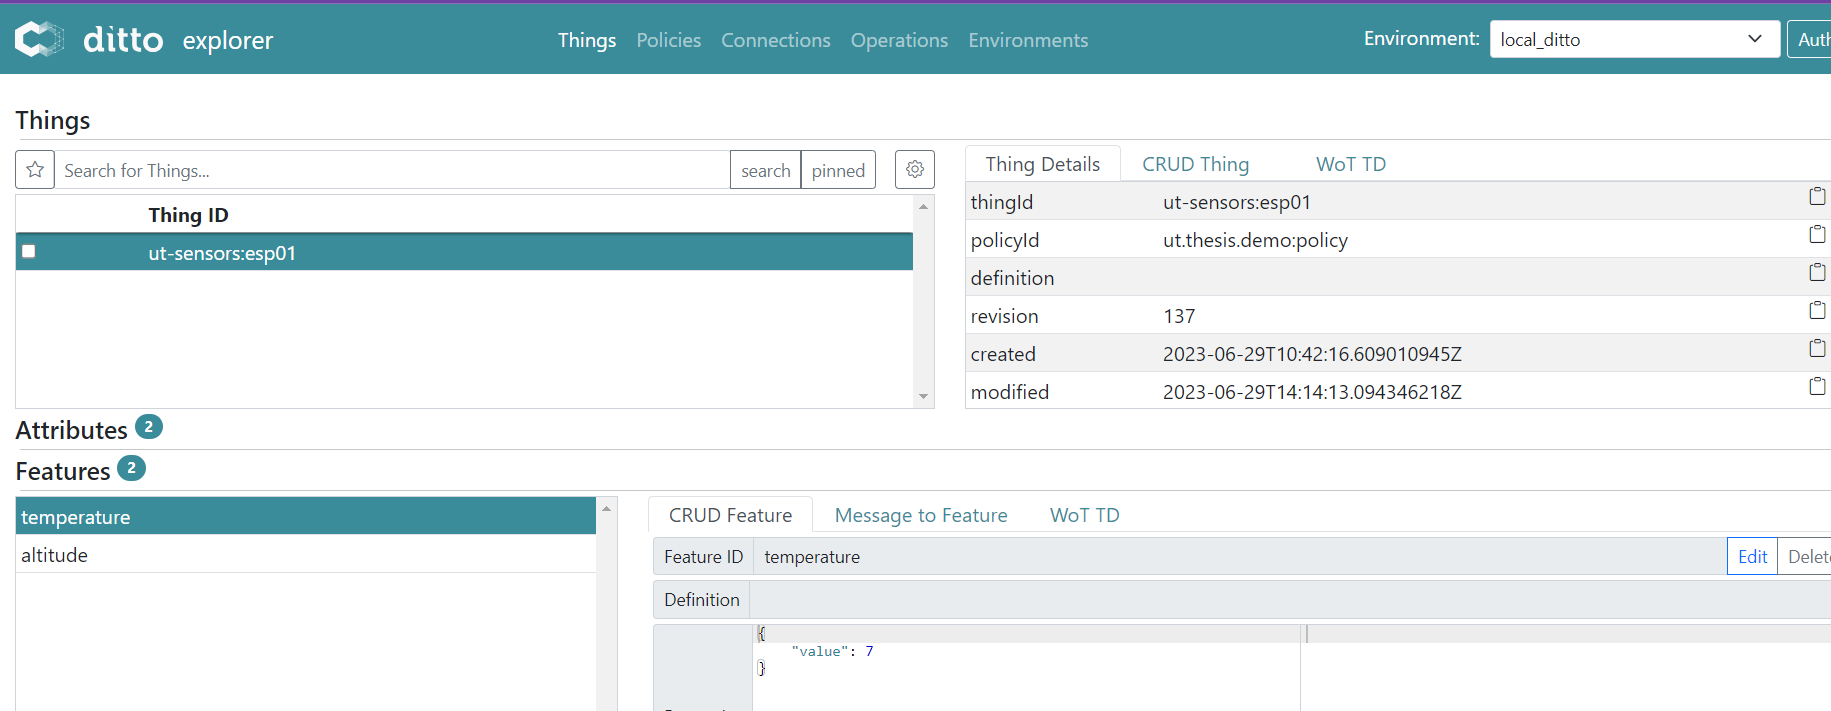
\includegraphics[width=\linewidth]{images/fp/ditto-log.png}
        \caption{A Data Log Viewed from Ditto Platform}
        \label{fig:ditto-log}
    \end{subfigure}
    
    \begin{subfigure}[c]{1\linewidth}
        \centering
        
        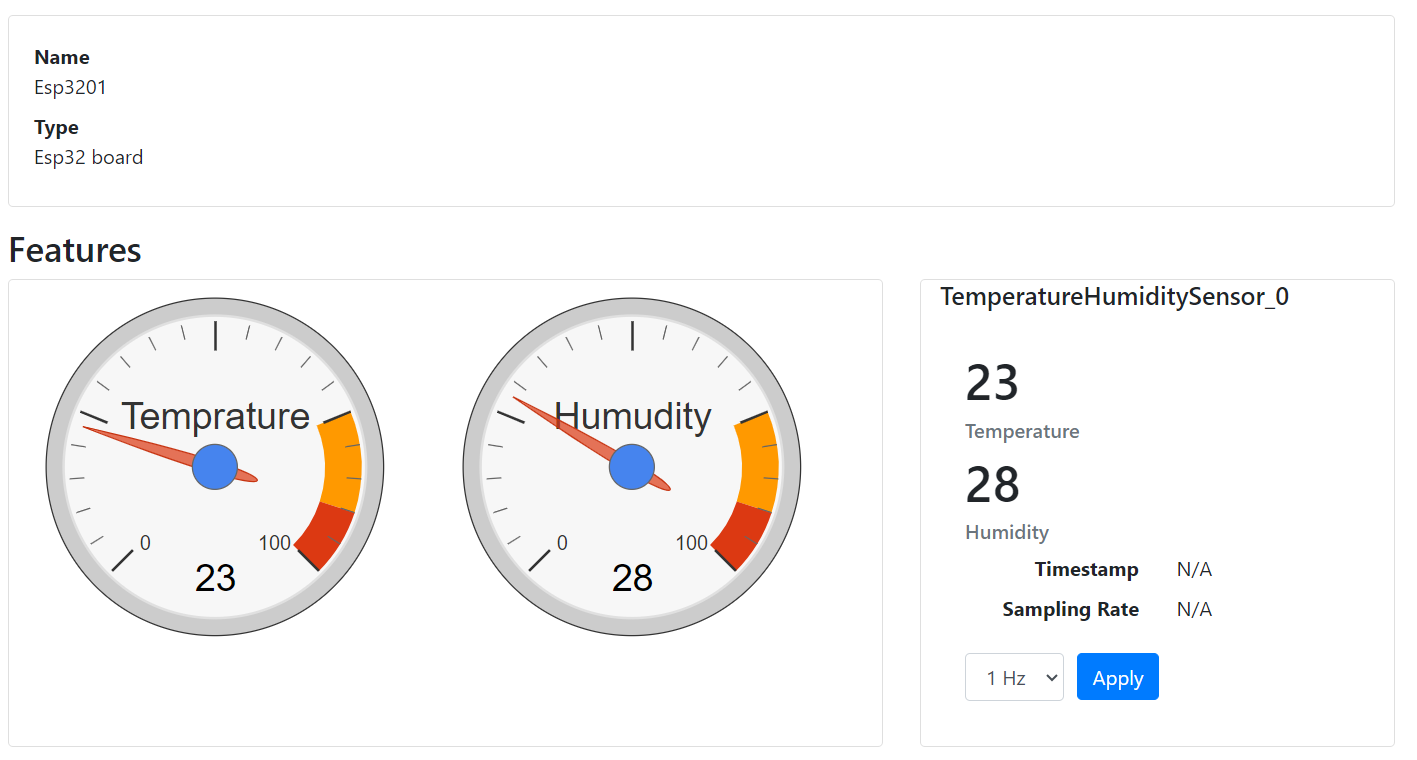
\includegraphics[width=\linewidth]{images/fp/appgauge.png}
        \caption{Web Application For Modeling Temperature and Humidity of ESP32}
        \label{fig:appdt}
     \end{subfigure} 
      \caption{Ditto and Webapp Toward Simulating Digital Twin}
    \label{fig:ditto-app}
\end{figure}

Figure \ref{fig:ditto-log} illustrates the WebUI of Ditto, which is included by default in the code base. This web portal serves as a portal offering device, policy, and connection management functionalities. Additionally, Figure \ref{fig:appdt} provides an overview of an application layer built on the Digital Twin concept. The attributes displayed on the upper part of the image represent the name and type of the simulated device. The gauges visually represent the received device features, while the bottom right section presents textual information associated with the device.

 
In this chapter, we discussed the relevant background information, the design requirement of the proposed solution and the implementation details. By implementing the proposed solution on both the Digital Twin (Ditto) and (I)IoT device (ESP32) we show how to secure the communication channel using a resource-efficient authenticated encryption algorithm. 

In the next chapter, we provided performance analysis results of our proposed solution in terms of speed, memory usage and power consumption. For the analysis, we measure the performance of three implementations which are without an encryption algorithm, with ASCON, the recent winner of NIST lightweight encryption competition, and AES-GCM, AES-based authenticated encryption with associated data algorithm. 